% \section[CONCLUSIONS AND FUTURE WORK]{CONCLUSIONS AND \\ FUTURE WORK} \normalfont

\section[FUTURE WORK]{FUTURE WORK} \normalfont

\setlength{\epigraphwidth}{3in} 
\epigraph{\textit{We can only see a short distance ahead, but we can see plenty there
that needs to be done.}}{Alan M. Turing, Computing Machinery and Intelligence}

% Final conclusions, what does your research means? 

% And now it begins. no, now it ends. 

%%%%%%%%%%%%%%%%%%%%%%%%%%%%%%%%%%%%%%%%%%%%%%%%%%%%%%%%%

\setlength{\parindent}{0.0em}

% \begin{dissQuote}{\~{}Margaret Boden, The Creative Mind: Myths and Mechanisms, pp. 58}
%     We all test the rules, and consider bending them; even a saint can appreciate science fiction. We add constraints (lucky numbers?), to see what happens then. We seek the imposed constraints (only two numbers to be added), and try to overcome them by changing the rules. We follow up hunches ('Let's do subtraction, too'), and - sometimes - break out of dead-ends. Some people even make a living out of pushing the existing rules to their limits, finding all the computational 'cans' that exist: creative tax-lawyers call them loopholes (and creative tax-legislators close them).
% \end{dissQuote}

% \setlength{\epigraphwidth}{4in} 
% \epigraph{\textit{We all test the rules, and consider bending them; even a saint can appreciate science fiction. We add constraints [...] to see what happens then. We seek the imposed constraints [...] and try to overcome them by changing the rules. We follow up hunches [...], and - sometimes - break out of dead-ends. Some people even make a living out of pushing the existing rules to their limits, finding all the computational 'cans' that exist: creative tax-lawyers call them loopholes (and creative tax-legislators close them).}}{Margaret Boden \\ The Creative Mind: Myths and Mechanisms, pp. 58}

% \setlength{\epigraphwidth}{3in} 
% \epigraph{\textit{We can only see a short distance ahead, but we can see plenty there
% that needs to be done.}}{Alan M. Turing, Computing Machinery and Intelligence}

% % Final conclusions, what does your research means? 

% % And now it begins. no, now it ends. 

% %%%%%%%%%%%%%%%%%%%%%%%%%%%%%%%%%%%%%%%%%%%%%%%%%%%%%%%%%

% \setlength{\parindent}{0.0em}

% %This thesis explored~\acrshort{mi} collaboration between human designers and AI for the co-creation of games in~\acrshort{edd}, a~\acrshort{micc} system. The focus has been on developing techniques and algorithms to investigate this interaction to highlight and argue for the benefits that can be achieved. Specifically, mutual inspiration to explore unknown design areas, foster the designer's creativity, and establish adaptive experiences. 

% This thesis explored game design and the creation of game content through human-AI collaboration. We used EDD, and its inner extended systems (QuestGram, TropeTwist, and Story Designer) to analyze and study \acrshort{mi} collaboration. The focus has been on developing techniques and algorithms to investigate this interaction to highlight and argue for the benefits that can be achieved. Specifically, mutual inspiration to explore unknown design areas, foster the designer's creativity, and establish adaptive experiences. 

% \setlength{\parindent}{0.9em}

% The performed studies have shown how Quality-Diversity algorithms, grammars, and pattern-based approaches are promising approaches to generate game content and to be used by computational designers to collaborate with human designers in an MI-CC paradigm. Particularly, QD-algorithms and IC MAP-Elites, showed to be robust, stable; and when interacted with, had adaptive properties tha benefit both the human designer and the algorithm.

% The performed studies have shown that the use of game design patterns and pattern-based PCG is a promising approach to understand and to generate game content. The use of game design patterns have been applied on a different level than previously. Moreover, it has been demonstrated how design patterns instances at different levels: micro-, meso- and macro-patterns can be used for generation of game content. Closely tied to this is the use of patterns together with different approaches to pattern-based PCG. Finally, the empirical studies show that the proposed methods perform better than existing PCG methods in many respects.

% all the developed systems within s MI collaboration 
% This thesis dived into the essential question of how to create tools where human designers can have a \emph{colleague} partnership and collaboration with the AI, the properties that arise from this, and ways to enhance the collaboration, several if not more areas remain open.

% Furthermore, the interaction between designers and AI arises multiple dynamic properties such as initiative, control, and expressivity. \emph{Initiative} relates to how either agent engages in the tasks and to what extent. \emph{Control} relates to the control mechanisms enabled for either agent to direct or constraint the output of other agents based on some criteria. \emph{Expressivity} relates to the diversity of solutions that can be created by either agent.



% One of this thesis's objectives was to develop algorithms that could collaborate with designers, giving them a varying degree of control through control mechanisms while still being expressive (RQ1). Three control mechanisms were introduced where the designer had direct and indirect control over non-intuitive parameters of the~\acrshort{ea}. These were: \emph{Locking tiles}, \emph{designer's design}, and \emph{feature dimensions}. In \textsc{paper i}, an explorative study was carried out to evaluate~\acrshort{edd} and it's current functionalities with game developers to gather and analyze game designer's requirements and impressions. \textsc{paper ii} focused on introducing aesthetic criteria to evaluate the content, and as a way for the designer to preserve their content. The locking tiles feature was introduced, which allowed designers to designate their design areas to be preserved by the~\acrshort{ea}. This allowed the computational designer to be more supportive by focusing on parts that the designer was not currently working on.

% Moreover, a strong candidate to cope with both the control and expressivity dynamic properties that arise in the interaction are~\acrshort{qd} algorithms. Thus, in \textsc{paper iii} it was introduced and implemented the~\acrlong{icmape}, a variation of the~\acrshort{mape} algorithm. Among its features, it enabled the designer to select feature dimensions (a key component of~\acrshort{mape}, explained in section~\ref{sec:map-elites}). The results from \textsc{paper iii} pointed towards enabling enough control since selecting feature dimensions and their granularity changes the search landscape and the retained solutions. However, this changes the features a designer might be interested in but does not limit the algorithm's expressivity to create diverse solutions. Further, the fitness function of~\acrshort{icmape} continuously adapts to the designer's design, acting as an indirect control mechanism.

% The results from \textsc{paper iii} are further supported by preliminary results, where the behavior and generative space of~\acrshort{icmape} was analyzed by simulating design sessions. Given that one of the designer's interactions is the automated adaptation of the fitness based on the current design, we examined and evaluated how the search varied and adapted to a design session. The results show that the algorithm adapts adequately, and the designer has, to some large extent, an impact in the generative space with their design. More exciting is that~\acrshort{icmape} is able to explore new areas of the space by adapting to the designer's design. This result can be seen in figure~\ref{fig:FigureRejectedPaper}. 

% In short, controllability, in many cases, is a competing property with expressivity. Since the control and constraints imposed usually limit the expressive range for any of the constrained agents. However, in this thesis, it is demonstrated that~\acrshort{qd} algorithms, specifically,~\acrshort{icmape}, can cope with this, showing robustness, adaptability, and stability when interacted. It was provided meaningful control for the designer, yet~\acrshort{icmape} adapted and kept exploring vast amounts of the generative space encountering high-performing solutions. 

% \begin{figure}[t]
% \centerline{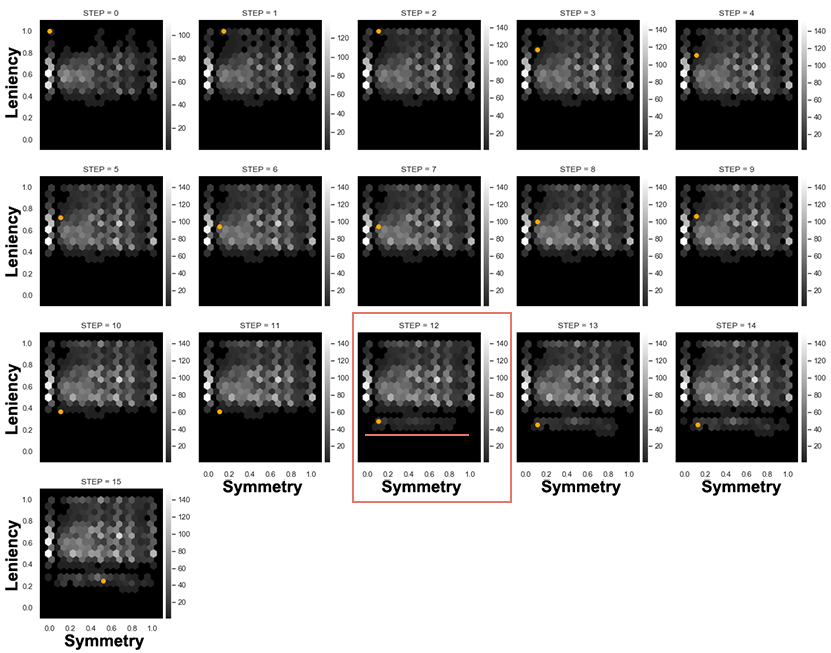
\includegraphics[width=\textwidth]{figures/ICMAPE-figs/accumulative__X-sym-Y-len-2.png}}
% %\centerline{\includegraphics[width=0.55\textwidth]{figures/low-len/accu__X-sym-Y-len.png}}
% \caption{Aggregated Expressive Range Analysis using Symmetry and Leniency as feature dimensions. The orange dot represents the designer's design that each step is edited and moving in the generative space. In step 12, it is highlighted the step when the designer's design enters a new generative area, which helps~\acrshort{icmape} explore the new area.}
% \label{fig:FigureRejectedPaper}
% \end{figure}

% Moreover, the work in \textsc{paper i, ii, ii} and the interest on seeking alternative approaches to foster creativity, to create adaptive experiences, and to enable more autonomy and initiative for the AI directed the research towards player and designer modeling. The former was explored in \textsc{paper iv}, where personality-driven player models were created to investigate their usability as a representative surrogate model and possible complement value in gameplay. 

% % Designer Modeling was explored through \textsc{paper v, vi}.
% \textsc{paper v} and~\textsc{paper vi} presented examples of designer modeling by modeling different designers' procedures. These could be used as surrogate models to enhance the understanding of design processes and the usability of design tools, such as~\acrshort{edd}. \textsc{paper v} presented a clear artifact design used to steer the generation of new suggestions based on the \textit{in situ} created preference model. This work demonstrated the benefits that come with integrating these models in the~\acrshort{mi} loop, such as the possibility of seamlessly creating preferred content. However, it also demonstrated the challenges of selecting and collecting representative data or training-and-using models as designers develop.

% Furthermore,~\textsc{paper vi} presented the development of a novel model to analyze the designer's design process, which could inform generative processes on the designer's style, goal, and intentions. The analysis of the resulting clusters based on each designer's design process resulted in the designer personas. These designer personas were presented as archetypical paths taken by designers through the clustered style space. Both models allow for the analysis of design and creative processes from an abstract level rather than specific steps, akin to procedural personas or game design patterns. 

% These approaches towards designer modeling have shown the capabilities of modeling several procedures and how they could be used. They also show that design processes can be analyzed more abstractly, yielding interesting similarities among seamlessly different designers or design processes. Designer modeling has the possibility to create adaptive experiences for an individual or group of designers and could enable more autonomy and initiative for the AI. However, whereas this, and its usability as surrogate models to enhance the collaboration, interaction, and generation produce actual benefits to the dynamic workflow of~\acrshort{micc} tools remain open for exploration as a promising area.

% If the aim of this research area is to push harder for mixed-initiative tools, where more autonomy is given to the AI, and for humans to consider the AI as a colleague as described by Lubart~\cite{LUBART2005-computerPartners} and Guzdial et al.~\cite{Guzdial2019-AISystemDesign-Creators} that can be taken serious and used its input as a key factor in the development of any type of content. Then we are required to develop AIs and tools that not only provides interesting and valuable input to the human, but also adaptive experiences that 

% \subsection{Future Work}

The work in this thesis had an ambitious overarching objective, which was partly explored, but that revealed many more exciting areas and paths to continue exploring.

% The work in this thesis explored MI-CC, its properties, and game design b

% \textsc{RQ1} was partly addressed by introducing and implementing~\acrshort{icmape} in~\acrshort{edd}, and exploring its use to generate different type of content, . However, it is necessary to examine the behavior of~\acrshort{icmape} when used for this interaction. These behaviors could be: how the generative space is affected by the design sessions, the combination with designer modeling, or how dynamic feature dimensions (e.g., similarity and inner similarity) affect the expressiveness of the algorithm.~\acrshort{pcg} through~\acrshort{qd} was proposed recently~\cite{gravina_procedural_2019}, pointing towards the interesting avenues that are approaching, and as discussed in this thesis, the many possibilities they have when introduced in human-AI interaction and collaboration.

% Furthermore, two approaches have been proposed to model different designer procedures as designer modeling, but more work needs to be in place to operationalize the findings and models. For instance, using and transforming the designer personas and the design style clustering presented in \textsc{paper vi} into an applicable model to study designers and their design and creative process. Moreover, how to use these models to steer the generation of content and create adaptive experiences remains open, as the interaction with designers is dynamic and heterogeneous.

\subsection{Human-AI Collaborative Properties}

This thesis has emphasized controllability as a core property in MI-CC systems that needs to be taken into consideration. We have argued that control can come at the expense of expressivity but with the aim of adaptability towards the designer. Using IC MAP-Elites, we have shown that not only expressivity does not need to be hindered by this, but that control can be a win-win situation for both the designer and the algorithm. However, these properties: ``controllability,'' ``expressivity,'' or ``adaptability,'' miss much of their nuance and their usability when taken as overarching properties. For instance, how can we calculate ``controllability'' or ``adaptability,'' and what would that mean? What would it mean to be 30\% percent adapted? These questions highlight the problem that these properties encompass too much meaning and require to be broken down and explored deeper. For instance, ``controllability'' could be explored on how control varies when this is direct or indirect; or when applied to the process, the product, or the other agents; or how it affects and changes the role of each agent. Exploring how these properties can be broken down and how to analyze systems with them to move towards deeper and more developed interactions and collaborations is an exciting open research area.

% Find those critical points where AI needs to (1) change role, (2) adapt, (3) take more control/agency/initiative. Basically identify designer's intentions.

% \begin{itemize}
%     \item Controllability
%     \item explainability
%     \item Adaptability
% \end{itemize}

\subsection{Designer Modeling and Adaptive Experiences}

%Find those critical points where AI needs to (1) change role, (2) adapt, (3) take more control/agency/initiative. Basically identify designer's intentions.

Two approaches have been proposed to model different designer procedures as designer modeling, but more work needs to be in place to operationalize the findings and models. For instance, using and transforming the designer personas and the design style clustering
presented in \textsc{paper ix} into an applicable model to study designers and their design and creative process. Moreover, how to use these models to steer the generation of content and create adaptive experiences remains open, as the interaction with designers is dynamic and heterogeneous.

Another interesting future work would be to use these adaptive models to identify and understand the designers' intentions. By knowing the designer's intentions and their current design process, one could adapt and tailor the system towards their needs. For instance, it would be important to find the critical points in the design process where AI could need to change role, adapt the generated content, or take more control, agency, or initiative.

%Adapting towards their intentions could help 

\subsection{Explainable AI}

To establish an in-depth relationship between human and AI, trustworthiness is also required from the AI, in order to give more autonomy, responsibility, and initiative to the AI in creative tasks. Explainable AI is a research field that aims at increasing the transparency of AI systems, making AI systems more accessible and more understandable~\cite{adadi_peeking_2018,doshi-velez_considerations_2018}.

Zhu et al.~\cite{zhu_explainable_2018} proposed the field of eXplainable AI for Designers (XAID) as a human-centered perspective on MI-CC tools. This work discusses three principles of mixed-initiative, \emph{explainability}, \emph{initiative}, and \emph{domain overlap}, where the latter focuses on the study of the overlapping creative tasks between game designers and black-box PCG systems in mixed-initiative contexts. Xie et al. present an example of this~\cite{xie_interactive_2019}, where they explored visualization techniques through an interactive level designer tool called \textit{QUBE} to explain and introduce machine learning principles to game designers.

% However, given the collaborative nature of the tasks and relation that human and AI have in these settings, there is the possibility that through Human-AI collaboration \emph{explainability} could be intrinsic to the collaboration. As humans explore and try different alternatives with these algorithms and models (e.g., virtual thinkering), better understanding and interpretation from how these models work could be achieved such as in~\cite{xie_interactive_2019}. Zhu et al.~\cite{zhu_player-ai_2021}

% Zhu et al.~\cite{zhu_player-ai_2021} explore connections between gameplay and AI-human interaction, arguing that “AI as play can expand current notions of human-AI interaction, which are predominantly productivity-based.” They suggest using play to help people discover capabilities of an AI-enabled tool.

% \textbf{Digital thinkering}

% \emph{Thinkering}, the idea of doing something with yuor hands 

\subsection{Holistic Procedural Content Generation}

In this thesis, we scratched the surface of holistic PCG and its implementation in MI-CC systems. Whole systems, where facets are not only intertwined, but designers can start the design process from any of them, is a very interesting path. If designers were able to start by designing quests or objectives, and the system could adapt to these and generate levels or structures to support these or vice versa, MI-CC tools would be more aligned with how design processes start. These do not often start from the same starting point but tend to vary, and allowing that variance might be necessary to have different and more fruitful creative experiences. The system would then be in accordance with both Dehn’s definition, that space (world) is developed as post hoc justification for events by authors~\cite{dehn_story_1981}, and with Lebowitz, that the story gives meaning to a created world~\cite{lebowitz_creating_1983}. 

% An interesting and exciting path would be to explore the concept of holistic~\acrshort{pcg} and orchestration of the different game facets~\cite{liapis_orchestrating_2019} in connection with the~\acrshort{mi} paradigm. Holistic~\acrshort{pcg} is the generation of multiple contents (in different game facets) fitting each other in harmony as a collaborative process akin to how games are developed, with a limited amount of examples, but exhibiting exciting results~\cite{hartsook_toward_2011,cook_rogue_2014,hoover_audioinspace_2015,smith_situating_2011,dormans_generating_2011}. However, to what extent the generation is created in such a harmony that the facets interact and affect each other, and to what degree the user can interact with it is an open area for active research. 

% Furthermore, there exists an essential link and relation between space (e.g., level or objects within) and narrative (e.g., the story tried to be told). Thus, choosing and associating level design and narrative as two facets to explore within the holistic~\acrshort{pcg} approach is appropriated. This was presented and described by Kybartas and Bidarra's survey~\cite{kybartas_quinn_survey_2017}, and explored and supported by related work~\cite{kishino_hunt_2005,dehn_story_1981,lebowitz_creating_1983,hartsook_toward_2011,karavolos_mixed-initiative_2015,abuzuraiq_taksim_2019}. Within the narrative facet and in most games, quests are an essential component. Therefore, exploring and generating quests is paramount by exploring multiple quest concepts~\cite{yu_what_2020}, analyzing quest patterns~\cite{trenton_quest_2010,smith_situating_2011}, and using surrounding ideas such as kernels and satellites for event division~\cite{aarseth_narrative_2012}.


%using different denifitions~\cite{yu2020quest}, Within the narrative facet as well as in most games, quests are an essential componen I want to add this work by Yu et al.~\cite{yu2020quest}

% It is paramount to identify the roles, goals, conflicts, relations that exist in a narrative scenario 
%Quests have been studied 

% Thus far, some exploratory work has been done combining both facets in the generative process of~\acrshort{edd}. Firstly, through a simple but effective way of analyzing patterns and objectives created by designers when designing their levels~\cite{flodhag_make_2020}. Secondly, by introducing~\acrshort{mi} creation of quests using grammars based on the quest analysis by Doran and Parberry~\cite{doran_prototype_2011}, to compose a series of subsequent objectives together with the designer~\cite{alvarez_questgram_2021}. 

% Therefore, having this as a base and using the current findings in this thesis, the aim is to explore the~\acrshort{micc} paradigm applied to holistic~\acrshort{pcg} through the following RQ and subRQs (continuing the numbering from the RQs presented in this thesis): 

% \begin{itemize}
%     \item[] \textbf{RQ4.} How can level design and narrative interact, act as constraints, be intertwined, and in general, have an active role affecting each other, in order to, produce a holistic system?
%     \begin{itemize}
%         \item[] \textbf{RQ4.1:} What are the requirements and main factors needed to establish a relation between the level design and the narrative, and what are the criteria to evaluate the respective generated content? 
%         \item[] \textbf{RQ4.2:} What are the factors to be considered when implementing such a paradigm and system in a mixed-initiative application, where a designer will be able to interact with the content?
%         \item[] \textbf{RQ4.3:} What are the effects of producing and using a holistic system for the creative process of a designer, and what challenges are imposed on computational creativity? 
%     \end{itemize}
% \end{itemize}


\subsection{Exploring Agency and Initiative in Mixed-Initiative}

As paths towards adaptive experiences that recognize several designer procedures are explored, it is expected to establish the foundations of a deeper relationship between humans and AI. Through this thesis, control mechanisms were given to designers while not reducing the expressiveness of the AI. Further, examining and modeling different designer procedures, such as their design process, style, preferences, and goals as they create content, have enabled this thesis to explore important steps towards a mature relationship. It is hypothesized that this is needed to create more autonomy and initiative for the AI and to establish a trustworthy relationship between both agents, yet, this might not be enough. This thesis barely scratched the surface of the relationship, the possibilities that emerge with them, and the AI's initiative and role. In \textsc{paper xii}, we took the first steps toward altering the role and agency of both humans and AI, and had interesting results that still require much exploration. Therefore, another future direction is to explore varying autonomy, agency, and initiative for both agents and how that affects the interaction and design and creative process of the co-design and~\acrshort{mi} paradigm.

% This is compiled into the following RQ:


% is how varying the autonomy, agency, and initiative of t

% \begin{itemize}
%     \item[] \textbf{RQ5.} How does the agency of the designer and the agency of the computational designer in mixed-initiative approaches, and the interaction between both actors, affects the overall design process and the usefulness of mixed-initiative tools?
% \end{itemize}

% \subsubsection{Different Interactions}

% Finally, it is exciting to have explored all that this thesis present, but it is even more to see the road in front and realize all the paths that remain open and to be explored through future work.


% while this thesis has presented steps towards a better understanding through designer modeling and , it is especulated this thesis only especulates  has explored speculates that both of these research areas are needed to establish a trust relationship between both actors, yet, this might not be enough.

% Giving control to the designer while not reducing the expressive power of the AI, understanding different designer procedures such as their design process, style, and goals as they create levels, and modeling multiple subjective properties such as designers preferences and intentions; have enabled this thesis to explore interesting and important steps towards a mature relation. However, this thesis barely scratched the surface of the relationship and the possibilities that emerge with them. 

% Moreover, as it is explore paths towards adaptive experiences that recognize several designer procedures; we hope to establish the foundations of a deeper relation between human and AI. Giving control to the designer while not reducing the expressive power of the AI, understanding different designer procedures such as their design process, style, and goals as they create levels, and modeling multiple subjective properties such as designers preferences and intentions; have enabled this thesis to explore interesting and important steps towards a mature relation. However, this thesis barely scratched the surface of the relationship and the possibilities that emerge with them. 

% Moreover, as introduced in the problem statement (see section~\ref{sec:problemst}), it is required to have both an understanding from the AI of the multiple human procedures and an understanding from the human of how the AI system operates and it's decision process. In this thesis, this has been used and explained as Designer Modeling~\cite{Liapis2013-designerModel} and Explainable AI~\cite{Zhu2018-XAIDesignersMICC}. However, while this thesis has presented steps towards a better understanding through designer modeling, it is especulated this thesis only especulates  has explored speculates that both of these research areas are needed to establish a trust relationship between both actors, yet, this might not be enough. There are 


% As introduced in the problem statement (see section~\ref{sec:problemst}), it is required to have both an understanding from the AI of the multiple human procedures and an understanding from the human of how the AI system operates and it's decision process,  which translates to Designer Modeling~\cite{Liapis2013-designerModel} and Explainable AI~\cite{Zhu2018-XAIDesignersMICC}. However, such a system does not exist, and this thesis speculates that both of these research areas are needed to establish a trust relationship between both actors, yet, this might not be enough. There are 

% \begin{itemize}
%     \item[] \textbf{RQ5.} How does the agency of the designer and the agency of the computational designer in mixed-initiative approaches, and the interaction between both actors, affects the overall design process and the usefulness of mixed-initiative tools?
% \end{itemize}

% It is exciting to have explored all this thesis present, but it is even more to see the road in front and realize all the paths that remain open and to be explored through future work.
